\documentclass[a4paper,twoside]{article}

\usepackage{epsfig}
\usepackage{subcaption}
\usepackage{calc}
\usepackage{comment}
\usepackage{amssymb}
\usepackage{amstext}
\usepackage{amsmath}
\usepackage{amsthm}
\usepackage{multicol}
\usepackage{pslatex}
\usepackage{apalike}
\usepackage{xcolor}
\usepackage{multirow}
\usepackage{array}
\usepackage{SCITEPRESS}
\usepackage{graphicx} % Please add other packages that you may need BEFORE the SCITEPRESS.sty package.

\newcommand{\head}[1]{\textbf{#1}}
\newcolumntype{C}[1]{>{\centering\arraybackslash}p{#1}}


\begin{document}

\title{A Case Study on Performance Optimization Techniques in Java Programming}

\author{\authorname{Ciprian Khlud\sup{1}\orcidAuthor{0000-0001-6211-3199}
  and Cristian Fr\u asinaru\sup{1}\orcidAuthor{0000-0002-5246-7396}}
\affiliation{\sup{1}"Alexandru Ioan Cuza University", Ia\c si, Romania}
\email{ciprian.mustiata@gmail.com, acf@info.uaic.ro}
}

\keywords{Java, Runtime performance, Memory usage, Garbage collection, Sequence analysis, SAM/BAM files}

\abstract{
    In today's era of relatively many cores and high memory capacity in regular machines, developers have to look into
    many competing languages and technologies. Java is typically discarded as a high memory consumption platform even though the performance of the generated code is considered adequate.
    As a composite to memory consumption, high heap usage translates into long GC pauses and overall slower performance in some memory intensive applications that use tens of GB.
    This paper will explore that Java, albeit consuming more memory than the equivalent platform, that applications using common Java patterns of storing in-memory data in
    a way that is friendlier to Java runtime and give adequate performance.
    The two examples taken as examples are a
    and these techniques would scale from hundreds of MB upto tens of GB of RAM and we do this explor
}

\onecolumn \maketitle \normalsize \setcounter{footnote}{0} \vfill

\section{\uppercase{Introduction}}
\label{intro}

In today's era of multi-core machines with high RAM capacity it is harder to use these machines efficiently.
As a secondary requirement developers want to use commonly known languages that are easy to use and to make minimum compromises.

In fields like finance, bioinformatics, search engines, they require using a large in-memory data sets and perform various operations on it. In bioinformatics, there are common operations as sequence alignment, variant detection, search against biological databases, etc.

Many tools exist to perform these operations, most of them handling specific use cases and they have in common processor and memory intensive tasks: I/O operations on large file,
compression/decompression, text processing, etc.

Choosing a programming platform that offers all the required instruments to handle the specific challenges in
bioinformatics is important,
as pointed out in a recent study dedicated to migrating an existing Common Lisp application, called elPrep, 
to another platform with better support for memory management and concurrency~\cite{costanza:2019}.
ElPrep~\cite{herzeel:2019} is a multithreaded tool for preparing sequence alignment/map files (SAM/BAM)
for variant calling in DNA sequencing pipelines. 
A key feature of elPrep is the ability to avoid the standard practice of creating a pipeline consisting of multiple
command line tools invocations,
executing a single pass through a SAM/BAM file and keeping data as much as possible in main memory.
In~\cite{costanza:2019} the authors investigated Go, Java and C++ programming platforms, as an alternative to Common Lisp.
The result of their study concluded that the Go implementation performed best, using a metric that involved both the
RAM usage and the runtime performance.
The benchmarks of the study showed that Java had a faster runtime, but a significantly higher memory usage, while Go
offered a better balance between the two.

As the Java source code for elPrep is available at {\texttt{https://github.com/exascience/elprep-bench}}, this paper will
analyse various parts of Java Runtime, especially memory management and thread synchronization, and propose a series of improvements
that could increase significantly the performance of the Java implementation, up to the point that would show that Java would be
competitive with Go implementation via simple tunning and it will be even more dramatic improvements using more tuned Java techniques.

As a simpler use-case, it will be shown that  a simple ip location service would keep the actual IP location database in memory in a feasible way.

As the scale of these two applications is different (of around 2 orders of magnitude in memory usage, and in scalability requirements),
the techniques are showing a practical way for applications that are limited in memory usage or in GC.


\section{\uppercase{Background}}
\label{background}

\subsection{\uppercase{Garbage Collection}}
\label{background:gc}

In order to analyze the behavior of memory intensive applications, it is important to understand how garbage collection
works and especially how Java~\cite{java} implements its garbage collectors.

The Java Virtual Machine (JVM)~\cite{lindholm:2014} offers an automatic storage management system,
called {\textit{garbage collector} (GC)} which reclaims heap storage occupied by objects which are no longer used.
The garbage collection process~\cite{gc:oracle} works typically by splitting the heap into two regions:
a {\textit{young generation}} region and an {\textit{old generation}}.
All new objects are allocated in the young region, in a very fast manner, using typically a "bump-pointer" strategy.
When this region becomes full  a {\textit{minor}} garbage collection occurs and all dead objects are deleted very quickly.
The objects which are still referenced survive, and then they are moved to the old generation.
This minor collection is always a "stop the world" event, meaning that all of the application threads will be paused
until the GC is finished.
In the old generation, objects are expected to live longer and they are collected more seldom but with a more expensive
algorithm, called {\textit{major}} garbage collection.

The algorithm used by GC has two steps.
The first one is to {\textit{mark}} the objects that are still used from the heap.
In the second step, it {\textit{sweeps}  (deletes)} the objects which have not been marked (dead), leaving only
referenced objects and pointers to free space.
By moving referenced objects together, this makes new memory allocation much easier and faster.
Therefore, the speed of GC depends on two factors: the number of objects it has to analyze and the complexity of the
relationships between them.

Objects are allocated using {\textit{new}} operator, and by Java specification, these objects are allocated having an
8 byte alignment and it is also depending of the JVM bitness (64 vs 32 bit) there will be a fixed ovearhead used for
object's identity. This means that even an empty string literal or a Boolean (a wrapped box type) will have an overhead
that if repeated for many times (which is quite common in large data sets), it would become a significant overhead (as it will be shown).

Considering the behavior we have described so far, we will analyze the impact of some simple tweaks
meant to reduce the impact of GC over the application performance, such as:
reducing the unnecessary small allocations in young region, controlling the scope in which objects are referenced in
order to minimize the number of times when expensive collection of old region is triggered,
simplifying the object graph and controlling the amount of memory JVM is allowed to use.


\subsection{\uppercase{Memory Usage}}
\label{subsec:memory}

The Java Virtual Machine allocates memory either on stack or on heap~\cite{lindholm:2014}.

The {\textit{heap}} is the place where all class instances and arrays are allocated and it is shared among all threads.
Each JVM thread has a private {\textit{stack}} which holds local variables and partial results  during successive method invocations and returns.
When working with large amounts of objects it is quite important to assess the memory consumption of a data structure, in a manner similar to the {\textit{sizeof}} construct in C or C++.
An object allocated on the heap has a {\textit{header}} which contains information used for locking, garbage collection or the identity of that object.
The size of the header depends on the operating system, and it may be 8 bytes on 32 bit architectures or 16 bytes on 64 bit architectures.
Also, for performance reasons and in order to conform with most of the hardware architectures, JVM will {\textit{align}} data.
That means that if we have an object that wraps just one byte, it will not use: $8 \text{(object header)} + 1 \text{(content)} = 9 $ bytes of memory on the heap, but it will use $16$ bytes as it needs to be aligned to the next $8$ byte boundary.

In Java, strings are objects and they are allocated on the heap.
That fact that string literals are stored in a shared object pool, in order to reduce memory consumption, is of no relevance in our context.
Inspecting the source code of the \texttt{String} class, one can observe the following instance fields:
\begin{small}
\begin{verbatim}
private final byte[] value;
private final byte coder;
private int hash;
\end{verbatim}
%// Defaults to 0
\end{small}

As expected, a \texttt{String} object keeps a reference to an internal byte array.
However, the other two fields will make the size of the object equal to: $8$ (header) $+$ $4$ \texttt{value} reference $+$ $1$  \texttt{coder} value $+$ $4$ \texttt{hash} value $= 17$ bytes.
Being aligned to $8$ bytes, it will actually use $24$ bytes.
When creating many \texttt{String} instances (like millions of them, as in our case study), the extra information included in this class will add up, consuming memory and  triggering the garbage collector more often than necessary. 

We will show that replacing the \texttt{String} usage to the underlying \texttt{value} byte array will improve the performance of the application, and this approach should be implemented in every scenario that involves processing large amounts of text data.




\section{\uppercase{Representing the Data Store}}
\label{sec:model}

\subsection{\uppercase{The Row-Based Model vs Column-Based Model}}
\label{subsec:row}

The benefit of using Java is simplicity of programming and Java is defined around object creation and it comes bundled with collections like arrays as built-in the language, but also APIs to do common operations with them like filtering, mapping them and so on, which makes developers to use these APIs out of convenience.
But, when the data set is into hundreds of thousands of items (or in case of sequencing algorithms like ElPrep it can go well beyong 10 millions), the memory consumption can go fast quickly.

For the IP database that gives the geometric location, something like this can be defined as a good representation that a developer could choose and put them into an ArrayList<LocationRow>

\begin{small}
\begin{verbatim}
public class LocationRow {
	long ipLow;
	long ipHigh;
	String countryCode;
	String country;
	String region;
	String city;
	double latitude;
	double longitude;
	String zipCode;
}
\end{verbatim}
\end{small}

When storing these locations parsed out of a 2020 database of these fields and stored, the live memory (as live memory is the effective data that has to be allocated as minimum by the JVM, as various JVMs have different policies of allocation) consumption is quite high and let's understand why.

So let's see one instance's size of LocationRow: ipLow, ipHigh, latitude, longitude have $8$ bytes primitive types. $4$ strings of $24$ bytes each (not counting data) and $4$ (on 32 bit machines) bytes references and these String instances would have themselves a byte array, which itself starts from $16$ byte starting size and it will increase in increments of 8 every time a string exceeds 8 bytes long. But not considering the byte content we have the following overheads. And on top of this we have to add $12$ bytes object headers for the LocationRow itself
$ 4 * 8 + 4 * (24 + 4 + 16) + 12 = 220$

If multiplied by 2.8 million rows, the storing envelope (which contains some useful data, like the long/double instances) is around 600 MB. If stored in an ArrayList, the ArrayList itself has to store these $2.8$ million references of $4$ bytes which themselves add to another 11 MB.

Now let's flip the order of storing, and instead of keeping an ArrayList<LocationRow> we will have a repository class that will store the columns individually as follows:

\begin{small}
	\begin{verbatim}
public class LocationRowRepository {
    LongArrayList ipLow;
	LongArrayList ipHigh;
	DeduplicatedDictionary countryCode;
	DeduplicatedDictionary country;
	DeduplicatedDictionary region;
	StringSequence city;
	DoubleArrayList latitude;
	DoubleArrayList longitude;
	StringSequence zipCode;
}
\end{verbatim}
\end{small}

So we will store the all locations data in long sequences but the overhead is fixed per entire data set: every new row doesn't add many objects, so per every instance there are the following costs:
4 instances of 8 bytes (ipLow, ipHigh, latitude and longitude), 3 classes that use 2 bytes per string to identify commonly repeating names and city which uses extra 4 bytes to store the length of StringSequence (these collections would be detailed in the next section how they work)

So memory consumption per every row would be:
$4 * 8 +  + 3 * 2 + 4 = 42$

And combined envelope would be a fixed: 2.8 million * 42 bytes around 120 MB and added on top, some data would be deduplicated.

Similarly, for ElPrep algorithm instead of many {\texttt{SamAlignment}} instances, we will have a single object of type {\texttt{SamBatch}} which contains references to the "columns", ie our data structures holding all the information of a specific type.


Regardless of VM bitness, the memory consumption for representing one row of the input file is: 
\begin{center}
\begin{tabular}{ l l l }
 {\textbf{Data Type}} 				& {\textbf{Count}} 		& {\textbf{Bytes}} \\
 {\texttt{StringSequence}} 		    & $2$ 				& $4$ \\
 {\texttt{DeduplicatedDictionary}}	& $3$ 				& $4$ \\
 {\texttt{IntArraySequence}}		& $3$		 		& $4$ \\
 {\texttt{CharArraySequence}}		& $1$				& $2$ \\
 {\texttt{ByteArrayList}}			& $1$				& $1$ \\
 {\texttt{DnaEncodingSequence}}	    & $1$ 				& $4$ \\
 {\textbf{Total}}					& 					& $\mathbf{39}$
\end{tabular}
\end{center}

Considering that no rounding up is necessary, for $2.1$ million rows this sums up to $81,900,000$ bytes,
equivalent to $78$ MB. The header sizes of the column objects ($11*8$ bytes) become negligible in this context.

We will explain later, in section \ref{subsec:batching}, how additional memory savings ($2$ bytes per instance) can be achieved using {\textit{chunking} } and {\textit{batching} }, but for now, in order to have a visual description of the data representation, the following graph shows a comparison between the row-based and the column-based models (only for object bookkeeping and primitive values):

\begin{center}
	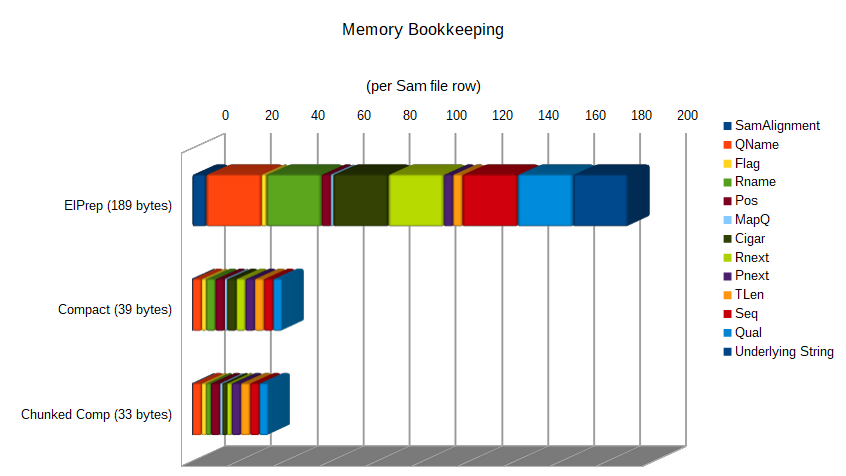
\includegraphics[scale=0.35]{images/MemoryBookeeping.png}
\end{center}



\subsection{\uppercase{Memory Compaction}}
\label{subsec:compaction}


As presented earlier, the collections are only storing their respective data, but the store of this data is
specialized for the type of the column, making changes more substantial.

{\texttt{StringSequence}} would store {\texttt{Strings}} instances that are not repeating often enough as follows:
\begin{verbatim}
String items[] = { "abc", "def" };
\end{verbatim}
each consuming memory due to their headers, we can use 
a single object of type {\texttt{String}}, storing all the characters, and an additional array for their lengths.
\begin{verbatim}
String dataPool = "abcdef";
int[] endLengths = {3, 6};
\end{verbatim}
The technique described above was implemented in the class {\texttt{StringSequence}}.

If the strings that are to be stored are repeated frequently, we can apply another optimization:
instead of keeping them joined, we will use an indexed collection containing all the distinct strings and an array holding one index for each string.
For example, {\texttt{\{} "abc", "def", "abc", "xyz", "abc"\}} becomes:
\begin{verbatim}
table   : {abc=>0, def=>1, xyz=>2}
items   : [0, 1, 0, 2, 0]
\end{verbatim}
The {\texttt{table}} structure is based on the class {\texttt{Object2IntOpenHashMap<String>}} from FastUtil library, instead of the standard {\texttt{HashMap<Integer, String>}}, since it uses the primitive data type {\texttt{int}} for representing the keys, which also saves some memory.
This data deduplication technique~\cite{he:2010},~\cite{manogar:2014} was implemented in the class {\texttt{DeduplicatedDictionary}}.

When storing strings containing characters from a restricted alphabet, one optimization that can be performed is using an array of primitive values, for example a {\texttt{long}[]}, and encoding each character into a block of bits.
The number of bits required for a character depends on the size of the alphabet.
DNA sequences use four letters {\texttt{A,C,G,T}}, but it is possible for a machine to read incorrectly a symbol and to return {\texttt{N}}.
In order to represent $5$ possible characters we need at least $3$ bits,
which means that a {\texttt{long}} can store in its $64$ bits $21$ DNA letters.
The class {\texttt{DnaEncodingSequence}} which implements this string encoding technique contains the following members:
\begin{verbatim}
LongArrayList content;
ShortArrayList lengths;      
IntArrayList positions;     
\end{verbatim}
For example, encoding the $21$ letters string "AAAACCCCGGGGTTTTNNNNA" would produce a single long value, containing the bits:\\
{\texttt{00001001001001000110110110110100
		10010010001001001001000000000000}
}

From right to left, $000$ represents A, $001$ represents C, and so on.

In the sample files, one DNA sequence is typically around $100$ letters, so the memory needed in order to represent it would be $1$ {\texttt{int}} (encoding length) and $5$ {\texttt{long}}s (the content), that is $44$ bytes.
This reduces the memory consumption by a factor of two.

Another advantage of using such an encoding is that when checking if two sequences are exactly the same, we can compare first their lengths and, if they are equal, comparing {\texttt{long}} values means evaluating $21$ characters at once.

{\texttt{TagSequence}} reduces drastically {\texttt{temps}} and {\texttt{TAGS}}  field and is implemented as a combination between {\texttt{StringSequence}} and {\texttt{DeduplicatedDictionary}}.
Since the {\texttt{tags}} are repeating frequently, we save them using one {\texttt{short}} value per tag, but instead of using a list of tags, we define a sequence of indices.

TagSequence does memory compaction by using a mix of short per-tag encoding and a full sequence of tags is joined together.

For the input {\texttt{"tag0 tag1 tag2", "tag1 tag2 tag3"}}, the representation would be:
\begin{verbatim}
table = {"tag0":0, "tag1":1, 
"tag2":2, "tag3":3},
lengths: [0,3], 
tagSequence = [0,1,2,1,2,3]; 
\end{verbatim}

The memory usage would be significantly improved (as expected), but the benefit is two fold: it makes GC pass to be called less often, because there is less memory allocated; and when the GC step happens, the number of objects is drastically smaller, so the runtime of GC would happen much faster.

Though a column store is a very good solution for size reduction, it has the downside of requiring more computational effort in order to work with multiple properties of the same object and deduplicate them.
However, when saving memory is the major concern, and especially when it comes to hundreds of GB per instance, the execution slowdown becomes far less important if we can achieve significant reductions in consumed memory.


\section{\uppercase{Optimizing JVM Operation on ElPrep}}
\label{sec:io}

\subsection{\uppercase{Buffering}}
\label{subsec:buffering}

Even the key step of improvement for ElPrep is memory compaction, given that the original algorithm
was stressing the GC (and this is shown in the ElPrep paper), it was spent time to find some bottlenecks
of the original elPrep Java implementation, and it was used to be a baseline.

When profiling ElPrep algorithm in Java, after the whole ElPrep algorithm is executed, in the writing writing step, the algorithm creates parallel tasks, which in turn take all \texttt{SamAlignment} instances and serialize them into the string format of SAM files.
Especially when the full data set is loaded into memory, these tasks create many small objects that have a negative impact in terms of memory management. Using a simple technique of {\textit{pre-allocating} } the buffer sizes based on the specific context of the problem, we can prevent the creation of many of these intermediate objects.

The code sequence that captures the writing process is presented below:
\begin{verbatim}
var outputStream = alnStream
  .parallel()
  .map((aln) -> {
    var sw = new StringWriter();
    try (var swout = new PrintWriter(sw)) {
      aln.format(swout);
    }
    return sw.toString();
});
\end{verbatim}

If we take a closer look at the {\texttt{StringWriter}} class we notice that it uses an internal {\texttt{StringBuffer}} object for storing its data, which in turn has an internal primitve buffer  ({\texttt{buffering} } \cite{oaks:2014}).
This buffer has an initial capacity and it is resized whenever the text that must be represented no longer fits into it. When the buffer is full, its capacity is doubled. 
The default size of a \texttt{StringBuffer} is $16$ characters, so creating a text of length $400$ would require $5$ resize operations, from $16$ to $512$. 

The average length of a row in the input file is $325 - 330$ characters.
As $350$ is about $10\%$ larger than the average line, based on the regular statistical distribution, this means that most lines would require no extra resizes of their corresponding buffers. This prevents the creation of extra garbage, which in turn reduces the number of times when GC is executed.

\begin{verbatim}
    var sw = new StringWriter(350);
\end{verbatim}
In the following sections, we will denote the algorithm that employs this technique as {\textit{PresizedBuffers} }.


\subsection{\uppercase{Synchronization}}
\label{subsec:sync}

Another bottleneck in the original ElPrep algorithm that is a more laborious to fix, is noticing
that the class that is used to write the ouput (PrintWriter) is internally synchronized, which makes that
even though elPrep is itself formatting in a multi-threaded fashion the formatted strings (from previous subsection).

Writing to the file is implemented by simply invoking the {\texttt{println}} method of a {\texttt{PrintWriter}} output stream, decorating a {\texttt{BufferedWriter}}, which in turns decorates a {\texttt{FileWriter}}.
\begin{verbatim}
var out = new PrintWriter(
  new BufferedWriter(
    new OutputStreamWriter(output)));
...    
outputStream.forEachOrdered(
  (s) -> out.println(s));
\end{verbatim}

Again, the {\texttt{PrintWriter.println}} method is using a {\texttt{synchronized}} block in order to fulfill its task, which is eventually an invocation to {\texttt{BufferedWriter.write}} method.
\begin{verbatim}
public void println(String x) {
  synchronized (lock) {
    print(x); println();
   }
}
\end{verbatim}
The {\texttt{BuffereWriter.write}} method is also synchronized and so is {\texttt{FileWriter.write}}, which is the last one invoked in this chain.

We did replace the writer code to a single-threaded version of the code that would be optimized and to avoid allocations and it is much faster as writing step. As to control allocation, instead of elPrep's Slice to store a String, the new algorithm will store the internal byte[], that in turn will make writing to disk directly and all other small changes that avoid allocations (so for example when reading integers in the row, the byte array/string is parsed character by character instead of using Java APIs that allocate.

These techniques will be referenced \texttt{StreamByteArray} algorithm.

\subsection{\uppercase{Column Store Compaction on Chunking-Batching and Extracting Parallelism}} 
\label{subsec:batching}

In the elPrep original algorithm, a {\texttt{SamAlignment}} object is created for each row in the input file.
In order to extract parallelism, there is an explicit {\texttt{.parallel}()} call, a construct that would create a task for each row that must be processed.
These tasks are queued and executed in a concurrent fashion using threads created transparently by the Java Stream API.
\begin{verbatim}
var alnStream = inputStream.parallel()
  .map((s) -> new SamAlignment(s));
\end{verbatim}
In the column-based model, described in section~\ref{subsec:column}, there is a single {\texttt{SamBatch}} instance storing all the data.
Because we perform data compaction, the {\textit{read}} operation must take into account the dependencies between rows. Just like in the case of removing duplicates, in order to process a new row we have to inspect the values of previously read rows and this means that the code between rows has to be single threaded.

In order to obtain a better performance than reading using a single thread, we propose a technique that splits the {\texttt{SamBatch}} structure in several "chunks".
Instead of having a single large object, we will represent the data using an array of smaller {\texttt{SamBatch}} objects.
A sketch of our {\textit{Compact}} algorithm is described by the following pseudo code:

\begin{verbatim}
int chunkSize = 20000;
int nbOfThreads = cpuCoreCount * 4;
var samBatches = new ArrayList<SamBatch>();
while (!endOfFile) {
  var rowsRead = parallelReadRows(
    batchSize, nbOfThreads);
  parallelTransformRowsIntoBatches(
    samBatches, rowsRead);
}
\end{verbatim}

The {\texttt{readRows}} method reads $chunkSize * nbOfThreads$ rows out of the SAM file for the next processing step.
The actual reading is done using an appropriate number of threads (based on the CPU configuration), each thread reading sequentially a fixed number of rows, calculated taking into account the nature of the information being encoded.
Having the data split into chunks, we can process in parallel the mapping between the associated text and the {\texttt{SamBatch}} data structure, where we perform data compaction and deduplication.
The technique of grouping similar tasks requiring the same resources in order to streamline their completion is called {\textit{batching}}.

In our case, the advantages of the chunking-batching approach are multiple:
\begin{itemize}
\item Transforming data, deduplicating and DNA encoding are all executed in a single-threaded manner, which is much easier to debug and understand than a multi-threaded equivalent.

\item Since a {\texttt{DeduplicatedDictionary}} will now have less than $20000$ unique strings, the values needed to encode the strings could be represented on $2$ bytes, instead of $4$.
Similarly, we can reduce the tag size from $4$ to $2$ bytes.

\item After the algorithm is fully executed,  we will have instead of $2.1$ million {\texttt{SamAlignment}} objects, about $105$ {\texttt{SamBatch}} instances, each of them having around $4$ orders of magnitude less objects overall.
This translates into $2$ orders of magnitude less objects.

\item When creating the output file, the {\texttt{SamBatch}} array could be processed in parallel, with no blocking except the actual operation of writing to disk.
\end{itemize}

We have seen that the column-based model saves memory at the expense of the running time.
This optimization, however, reduces the overall execution time of the read operation, which is now on par with the original implementation.

When it comes to writing, compared to our {\textit{StreamByteWriter} } algorithm, which is anyway much faster than the original implementation, the execution time is drastically reduced from $28$ seconds (for the $12$ GB BAM file) to $12$ seconds.
Preparing the strings that are to be written in the file can be done in almost perfect parallelism, using the available cores.
The only limitation remains the speed of output device, which can vary depending on its type: in-memory virtual partition, SSD, HD, etc.

In order to make sure there are no dead times when using the external device, it was also implemented the {\textit{async/await}} pattern. This allows the program to perform in advance reading operations, using a dedicated thread, while waiting for the data processing threads to complete their execution.
This new algorithm, called {\textit{Compact/Par}}, offers a small improvement in the running time, as we will see in the next section, but with the disadvantage of a significant increase in code complexity.

\section{\uppercase{Experimental Results}}
\label{sec:results}

\subsection{\uppercase{Overview}}
\label{subsec:overview}

We have created five implementations that address the most expensive parts of the elPrep algorithm, which are reading,  storing all data in the memory and writing.
Except for the original version, which was taken from elPrep public repository, all other algorithm implementations contain various types of optimization that are meant to improve runtime performance and to lower the memory usage, especially on large files where GC becomes a limiting factor. 
We recap the names of the algorithms as they are used in the following sections:
\begin{itemize}
\item {\textit{Original} }, the original algorithm described in~\cite{costanza:2019};

\item {\textit{PresizedBuffers} } {\textit{Original}} and the buffer of StringWriter is assigned with 350 characters by default, reducing GC load per row

\item {\textit{StreamByteArray} } transforms string into bytes and writes them directly into an \texttt{OutputStream}, reducing to almost zero the number of memory allocations related to writing.

\item {\textit{Compact} } employs a more elaborate column-based model for storing the data set in a "compact" form and uses specialised collections (i.e. deduplication)

\item {\textit{Compact/Par} } represents a modified variant of the {\textit{Compact} } algorithm aimed at reducing to a minimum the dead times regarding I/O operations.

\end{itemize}


The original elPrep benchmarks have been performed on a Supermicro SuperServer 1029U-TR4T node with two
Intel Xeon Gold 6126 processors consisting of 12 processor cores each, clocked at 2.6 GHz, with 384 GB RAM~\cite{costanza:2019}. The authors claim to do the processing of the 8 GB BAM file in 6 min:54sec to 7 min:31sec and memory usage is $330-340$ GB\@.

The computer we have used in order to perform the experiments is a Ryzen 9-3900X, having 12 cores and using 48 GB of RAM\@. Also, for smallest file we tested on a laptop with i7 4th gen with 4core and 16 GB of RAM.
Since we didn't have access to the hardware necessary to run all the tests in memory, as the original paper, we have used the smaller SAM files and ran the same processing repeatedly in order to obtain an accurate result of the running time, and writing the average time out of runs (after JVM was warmed up).

As we didn't have access to such a performing machine, we did most of testing with the smallest file, the $144$ MB BAM file ($673.3$ MB SAM file). For the $8$ GB BAM file ($27.18$ GB SAM) our results will show only the {\textit{Compact} } algorithm but we will make some inferences over the scaling of the algorithms across file sizes and cores.

For example, running $10$ times the algorithm on smallest input SAM file, which is approximately $700$ MB, will produce a total running time of around $70$ seconds (or 7 seconds per instance). 

Since the elPrep algorithm is designed to run everything in memory, we tuned the JVM heap size (using the \texttt{-Xmx} flag) to the maximum value allowed by the operating system. 

In order to analyze the performance of read/write operations, we made sure that no background OS services are running during our tests, by manually stopping them.


\subsection{\uppercase{Runtime performance}}
\label{subsec:runtimeperf}

The following table shows a brief comparison of the running times obtained by our algorithms, in three configurations: $144$ MB file using $4$ cores and $12$ cores, and $1.2$ GB file using $12$ cores. 

\begin{small}
\begin{center}
\textbf{Running time per algorithm in seconds} \\
\begin{tabular}{|C{2cm}|C{1.2cm}|C{1.2cm}|C{1.2cm}|}
\hline
						& 144 MB (4c)	& 144 MB (12c)		& 1.2 GB (12c)	\\ \hline
Original				& 9.13 			& 3.938 			& 123.91 		\\ \hline
PresizedBuffers			& 8.98 			& 4.19 				& 75.1 			\\ \hline
StreamByteArray			& 8.09 			& 3.43 				& 64.62 		\\ \hline
Compact 				& 5.64 			& 3.4 	 			& 34.5			\\ \hline
Compact/Par 			& 5.42		    & 4.68				& 26.7 			\\ \hline
\end{tabular}
\end{center}
\end{small}

The largest file shows the following numbers:
\begin{center}
	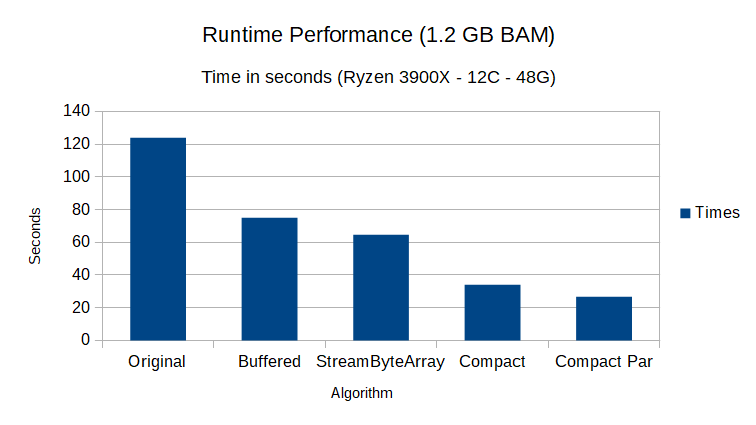
\includegraphics[scale=0.5]{images/runtime_perf_1_2G.png}
\end{center}

Comparing $4$ cores to $12$ cores, we notice that the {\textit{Original} } algorithm scales with a factor of $2.3$, {\textit{PresizedBuffers} } by a factor of $2.14$, {\textit{StreamByteArray} } scales by $2.36$ and {\textit{Compact} } would scale by $1.69$. So, at least for the small file, it seems that using larger machines will offer a better performance. It is important to notice that, in its current implementation, the {\textit{Compact} } algorithm has an explicit sequential part that reduces its scalability.
Some potential fixes are described in section \ref{sec:future}, where we describe some techniques aimed at improving the single threaded part.

A more useful way to present the algorithm is to show how it scales based on input size, and at least on the 12 core machine, we can see that both compact algorithms remain roughly in the same speed, so GC's runtime cost doesn't become in impediment:

\begin{center}
	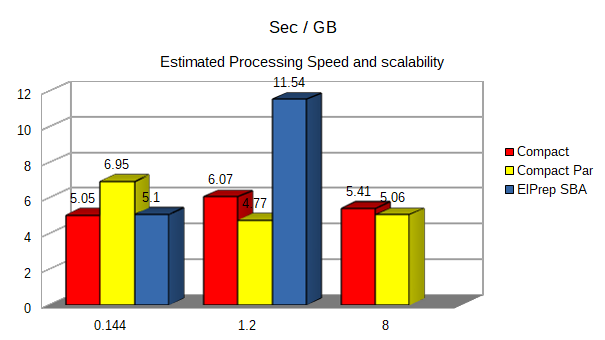
\includegraphics[scale=0.5]{images/seconds_per_gb_ryzen.png}
\end{center}



\subsection{\uppercase{Memory Usage}}
\label{subsec:memusage}
To measure the live data set, we have used Java VisualVM \cite{visualvm:oracle} which provides a visual interface for profiling a running application. Using VisualVM, we have analyzed the memory consumption in each scenario and we have estimated the minimum amount of memory that JVM requires in order to load a specific data set.

Unlike the original paper, which measures process's memory size, we have measured live data size as it avoids GC's algorithm specific allocation strateges and it is also important due to VisualVM which offers very precise information regarding the objects consuming memory.


\begin{small}
\begin{center}
\textbf{Memory usage per algorithm in MB} \\
	\begin{tabular}{|c|c|c|}
		\hline			  	& 144 MB file		& 1.2 GB file		\\ \hline
		Original			& 2326 MB			& 32025 MB			\\ \hline
		PreSizedBuffers		& 2326 MB			& 32025 MB			\\ \hline
		StreamByteArray 	& 2275 MB			& 31463 MB			\\ \hline
		Compact 			& 606 MB			& 4689 MB			\\ \hline
		Compact/Par			& 606 MB			& 4689 MB			\\ \hline
	\end{tabular}
\end{center}
\end{small}

Memory graphs look not so interesting, but the first two and last 2 columns are equal and on a similar note, the last 2 compact algorithms have the same 

\begin{center}
	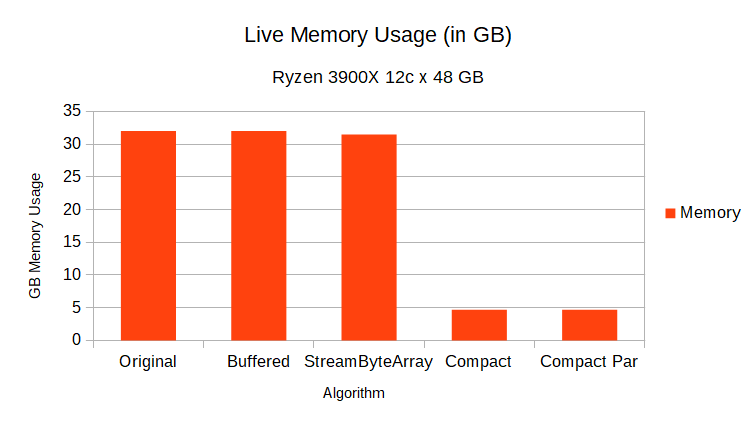
\includegraphics[scale=0.5]{images/memory_usage_1_2G.png}
\end{center}

Because the live memory usage is smaller than process's memory usage, there was no way to run on a 48 GB RAM machine the larger files.

On a $48$ GB machine, {\textit{Compact}} algorithms can process larger files: the $8$ GB BAM file uses $24283$ MB of live data and the $12$ GB BAM input uses $35 265$ MB.

We also have to note that not all of the used memory represents data related to the input file.
For example, in the case of the original elPrep algorithm, as it creates millions of tasks even for the smallest $144$ MB BAM file, Java Streams library will create a queue of objects that will remain in memory very likely until the end. This might add maybe around $100$ MB of memory, as it is quite hard (if not impossible) to measure it.

We also evaluated into an equivalent memory storage of other data set like the IP geolocation and we found that the memory usage is

\begin{small}
	\begin{center}
		\textbf{Memory usage of Geolocation DB in MB} \\
		\begin{tabular}{|c|c|}
			\hline			  	& IP location file		\\ \hline
			Original			& 932 MB			\\ \hline
			Compact 			& 212 MB			\\ \hline
			Compact/Par			& 171 MB			\\ \hline
		\end{tabular}
	\end{center}
\end{small}

Memory usage goes dramatically down, but it could be reduced even more, but the idea of compacting
column based store is very feasible for multiple use-cases: for example instead of country to use 2 bytes as deduplication, they can use 1 byte (as there are less than 256 countries), instead of float type a 24 bit latitude and longitude would be enough to store latitude and longitude value (using a 24 bit value, would translate into a precision of less than 3 meters, on equator), and so on.

\begin{center}
	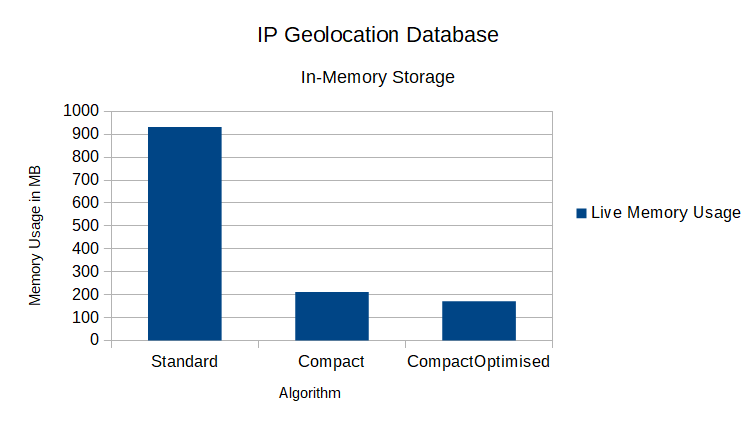
\includegraphics[scale=0.5]{images/Geolocation_Chart.png}
\end{center}

 
\subsection{\uppercase{Calculating Performance}}
\label{subsec:performance}
The goal of elPrep was to keep both the running time and the the memory consumption low. The evaluation function was defined as the multiplication of the average elapsed wall-clock time (in hours) with the average maximum memory use (in GB), with lower values (in GBh) being better \cite{costanza:2019}.
We have used the same approach, changing only the measurement units to MB and seconds.

In order to analyze the impact of the hardware to the performance of the algorithms, we have executed the tests on two distinct machines: the Ryzem 3900X ($1$2 cores and $48$ GB RAM).

On the medium file ($1.2$ GB BAM) the values are more conclusive from the point of view of scaling the results. We added for simplicity scaling said in original ElPrep's paper (the measurement they had was that Java implementation had a ratio that Go was around 76 percent of the Java score in the composite memory x runtime). The improvements resulting from our optimization techniques are now clearly visible. 

\begin{center}
	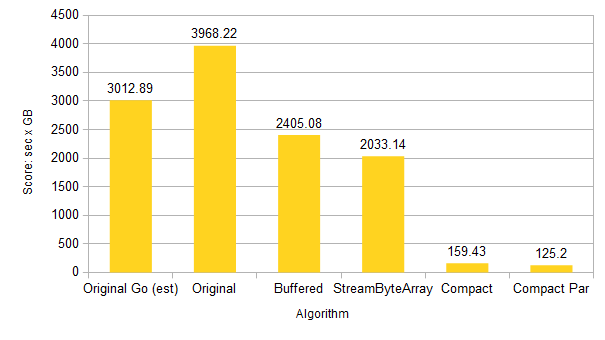
\includegraphics[scale=0.5]{images/times_and_memory_chart.png}
\end{center}


\section{\uppercase{Future work}}
\label{sec:future}

\textbf{Batch reader scalability} \\
As we have described in section \ref{subsec:batching}, our {\textit{batch reader} } works in two steps: initially, on the main thread, it extracts from the original file the rows for the number of the expected batches, and then it executes in parallel, using all cores, the data compaction step.
Before chunking and batching is done, we split the full byte array read from file into distinct  \texttt{List<byte[]>} instances.
This separation may not be necessary, an alternate approach being to store inside a large \texttt{byte[]} structure all the information and to use an additional array of indices in order to retrieve the actual lines of text.
This would reduce the number of allocations and eventually speed up the execution of the main thread.

A similar variation of speeding up the single threaded part is to not do the line splitting at all, but to read a block of text in advance, that would be around the expected chunk size,
and then split it in lines in a multithreaded way.

\textbf{Even more compacting} \\
The DNA sequence uses 3 bits per DNA letter, but in reality it could use just 2 for most sequences and use a flag to distinguish for the cases when letter N appears so to fall back to 3 bytes per letter. This could translate into a typically 2/3 less memory usage. 

\textbf{Value Types} \\
When Java specifications were elaborated, more than $25$ years ago, the cost of a retrieving an object from the memory and executing an arithmetic operation was approximately the same.
On modern hardware however, the memory fetch operations are up to $1000$ times more expensive than arithmetic ones.
This is why, the {\textit{Project Valhalla} } \cite{jdk:valhalla}, that is expected to be integrated in modern JDK releases, introduces new data structures and language constructs that improve various aspects regarding data manipulation.
For example, {\textit{Value Types} } provide the necessary infrastructure for working with immutable and reference-free objects.
In our context, this would allow us to further reduce the memory used by the {\textit{Compact} } algorithm by using an efficient by-value computation with non-primitive types.

\section{\uppercase{Conclusions}}
\label{sec:conclusions}
This paper addresses the situation when one has to manipulate a large textual data set by reading it from a file, transforming it into objects, processing it and then writing it back to a file, and all these operations must be performed in a single in-memory session.
We have analyzed a modern implementation of an algorithm for processing SAM and BAM files, elPrep \cite{herzeel:2015}, \cite{herzeel:2019}, which must handle input files up to $100$ GB. We also tested the benefits in memory usage into another more common services like an IP to location service that stores this data in memory and it is using Java.

The conclusion of the elPrep authors was that a Java implementation for this specific problem suffers from the memory management offered by JVM \cite{costanza:2019}.
However, when using an object-oriented programming platform, one has to take into consideration all aspects regarding memory allocation offered by that specific platform and to adapt its model and programming techniques.
Since Java is a general purpose programming platform, it offers a standard set of classes and language constructs providing a balance between performance and ease of use.
When dealing with hard problems, one has to analyze the default behavior of the programming interface and "tweak" it accordingly.

We have showed that even with small tweaks Java implementation of elPrep could even beat their original Go implementation.
We have showed that major improvements can be obtained by using techniques that are aimed at reducing the number of created objects.
This will not only save memory but it will also improve runtime performance by decreasing the overhead of the Garbage Collector.
Using a column-based representation we have compacted the data set in a manner that boosted the overall score calculated as the multiplication between used memory and running time.
The penalty incurred by the more elaborate data model was compensated by a multithreaded approach, called chunking-batching, that actually allows the algorithm to use all available machine cores when processing the input file.
In order to optimize the usage of the I/O device, we have also implemented the {\textit{async/await} } pattern, which also offered a small increase in performance.

Given the hardware differences between the machine used by the elPrep authors and ours, there are limits on the testing that could be done with the techniques used by this paper.
Instead of a $384$ GB of memory, dual-CPU server, we have used a machine  with $8$ times less RAM, half of CPU cores, a much slower disk drive (the SSD on the Ryzen machine can barely read at 300 MB/s, while a NVMe SSD can reach $32$ GB/s) and so on.
However, using input files ranging in size from $144$ MB to $12$ GB, we have proved that our algorithms are scalable and could perform as expected for files of any size, provided the machine has sufficient memory.





\bibliographystyle{apalike}
{\small
\bibliography{elprep-study}}


\end{document}

